% Photons:
%   explorer 11: 31
%   OSO-3: 621
%   SAS-2: ~8,000
%   COS-B: 

\section{The History of Gamma-ray Astrophysics}
\seclabel{history_gamma_ray_detectors}

It was only natural to wonder about photons with even
higher energies. These higher energy photons must
come from more extreme processes in space.

As is common in the field of physics, the prediction of
the detection of cosmic $\gamma$-rays far proceeded their discovery.
\cite{feenberg_1948_interaction-cosmic-ray} theorized that the interaction
of starlight with cosmic rays could produce $\gamma$-rays through
\ac{IC} upscattering.  Following the discovery of the neutral
pion in 1949, \cite{hayakawa_1952_propagation-cosmic}
predicted that $\gamma$-ray emission could be observed from the
decay of neutral pions when cosmic rays interacted with interstellar
matter.  And in the same year, \cite{hutchinson_1952_possible-relation}
discussed the bremsstrahlung radiation of cosmic-ray electrons.
\cite{morrison_1958_gamma-ray-astronomy} first predicted the detection
of several sources of $\gamma$-rays including solar flares, \acp{PWN},
and active galaxies.

Attempts were made in the 1940s and 1950s to determine the
composition of cosmic rays using balloon-based experiments. See,
for example \cite{critchfield_1952_radiation-balloon} and
\cite{hulsizer_1948_search-electrons}.  But the attempt to observe
cosmic $\gamma$-rays was hampered by the strong background of atmospheric
albedo $\gamma$-rays.

\begin{figure}[htb]
\centering
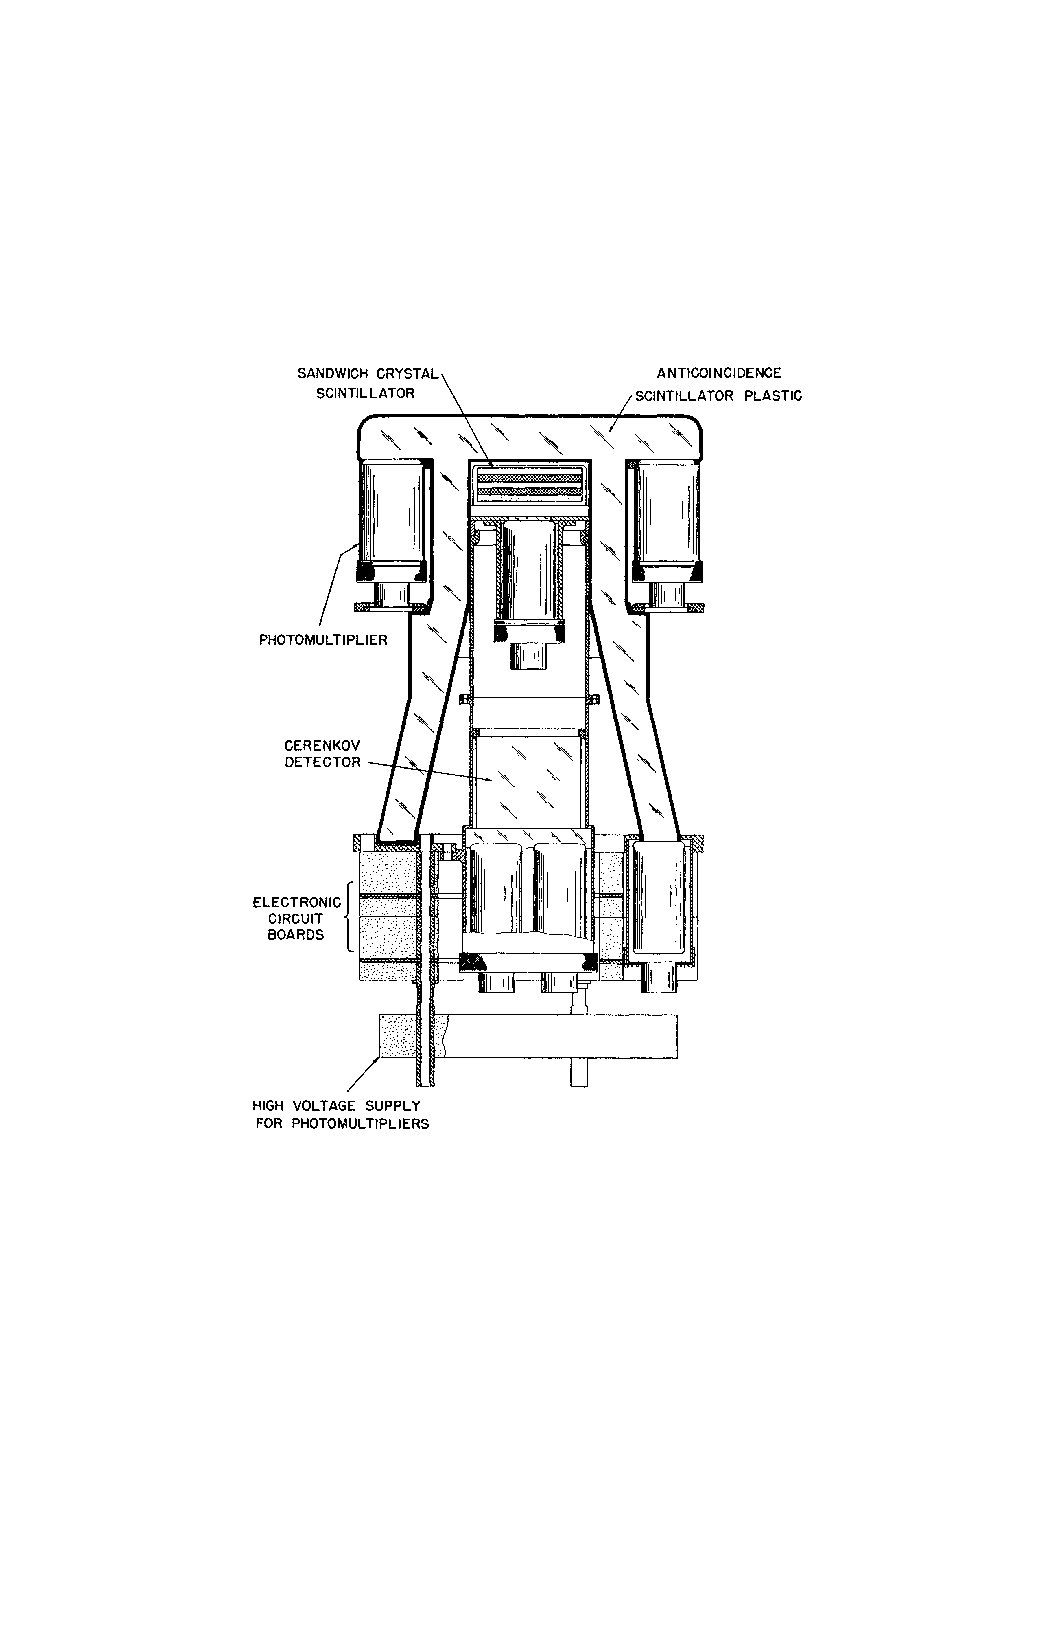
\includegraphics{chapters/introduction/figures/explorer_xi_instrument.pdf}
\figlabel{explorer_xi_instrument}
\caption{
The experimental design of \explorerxi.
This figure is from \cite{kraushaar_1965_explorer-experiment}. }
\end{figure}


    % Links on Explorer 11
% en.wikipedia.org/wiki/Explorer_11
%http://www.physics.wisc.edu/news/obits/kraushaar_obit.html
% http://heasarc.nasa.gov/docs/heasarc/missions/explorer11.html#reference
% http://articles.adsabs.harvard.edu/cgi-bin/nph-iarticle_query?1965ApJ...141..845K&amp;data_type=PDF_HIGH&amp;whole_paper=YES&amp;type=PRINTER&amp;filetype=.pdf

% "The instrument package weighed 30 pounds, was 20 inches high and 10 inches in diameter. The experimenters believed that they detected 22 cosmic gamma rays."
%  -> http://imagine.gsfc.nasa.gov/docs/sats_n_data/gamma_missions.html
The first space-based $\gamma$-ray detector was \explorerxi
\cite{kraushaar_1965_explorer-experiment}.  It was developed at \acp{MIT}
under the direction of William L. Kraushaar.  
\explorerxi incorporated five alternating slabs of cesium iodide and sodium
iodide which would induce a gamma-ray to pair-convert into an electron positron
pair. The electron and positron pair would then 
travel through
a sandwich scintillation detector.
A scintillator is a crystalline material that emits low-energy photons
when a high-energy charged particle travels through it.
A Cherenkov counter below the scintillation detector
measured these low-energy photons, which allowed
for the measurement of the energy of the
$\gamma$-rays.
This experiment was surrounded by a plastic anticoincidence
scintillation counter which allowed for the rejection of
background particles. \figref{explorer_xi_instrument}
shows the experimental design of \explorerxi.


\explorerxi operated in the energy energy range above $100\unitspace\mev$.
It had an area of $\sim45\cm^2$
but an effective area of only $\sim 7\cm^2$, corresponding
to a detector efficiency of $\sim 15\%$.

It was launched on board \explorerxi on April 27,
1961. The instrument was in operation for 7 months, but only 141 hours
of data were of acceptable quality.  Using these observations, \explorerxi
observed 31 $\gamma$-rays and, because the distribution a distribution of
these $\gamma$-rays was consistent with being isotropic, the experiment
could not firmly identify the $\gamma$-rays as being cosmic in nature.


% en.wikipedia.org/wiki/OSO_3
% "Their
% next detector, on Orbiting Solar Observatory -3, may be more accurately
% described as having proof of the discovery of cosmic gamma radiation,
% since it found a galactic plane anisotropy of high-energy gammas, much
% later to be confirmed with SAS-2 and COS-B." -- http://imagine.gsfc.nasa.gov/docs/sats_n_data/gamma_missions.html

% Notes: 621 photons, E>100 GeV, 1967, angular resolution +/- 16deg from 
%  ``Cosmic Gamma-Ray Sources`` K.S. Chen, Gustavo E. Romer

The first definitive detection of $\gamma$-ray came in
1962 by an experiment on the Ranger 3 moon
probe \citep{arnold_1962_gamma-space}.  It detected an isotropic flux
of $\gamma$-rays in the 0.5 \mev to 2.1 \mev energy range.

\Ac{OSO-3}, also developed by Kraushaar, 
was the next major astrophysical $\gamma$-ray detector
\citep{kraushaar_1972_high-energy-cosmic}.  \Ac{OSO-3} 
allowed the on board $\gamma$-ray detected to have an improved weight,
power, telemetry, and exposure, creating a more sensitive experiment.
The experiment operated in the energy range from 50 \mev to $\sim 400$
\mev, had an effective area $\sim 9$ $\cm^2$, and had a angular resolution of
$\sim 24\degree$ at its \ac{FWHM}.

\Ac{OSO-3} was launched on March 8, 1967 and operated for 16 months, measuring
621 cosmic $\gamma$-rays.  The most important result of the experiment was
to measure a strong anisotrophy in the distribution of the $\gamma$-rays
with a strong clustering of $\gamma$-rays towards the Galactic plane.
\figref{oso3_skymap} shows a sky map of these $\gamma$-rays.  This
experiment confirmed both a Galactic component to the $\gamma$-ray
sky as well as an additional isotropic component, hypothesised to be
extragalactic in origin.

\begin{figure}[htb]
  \centering
  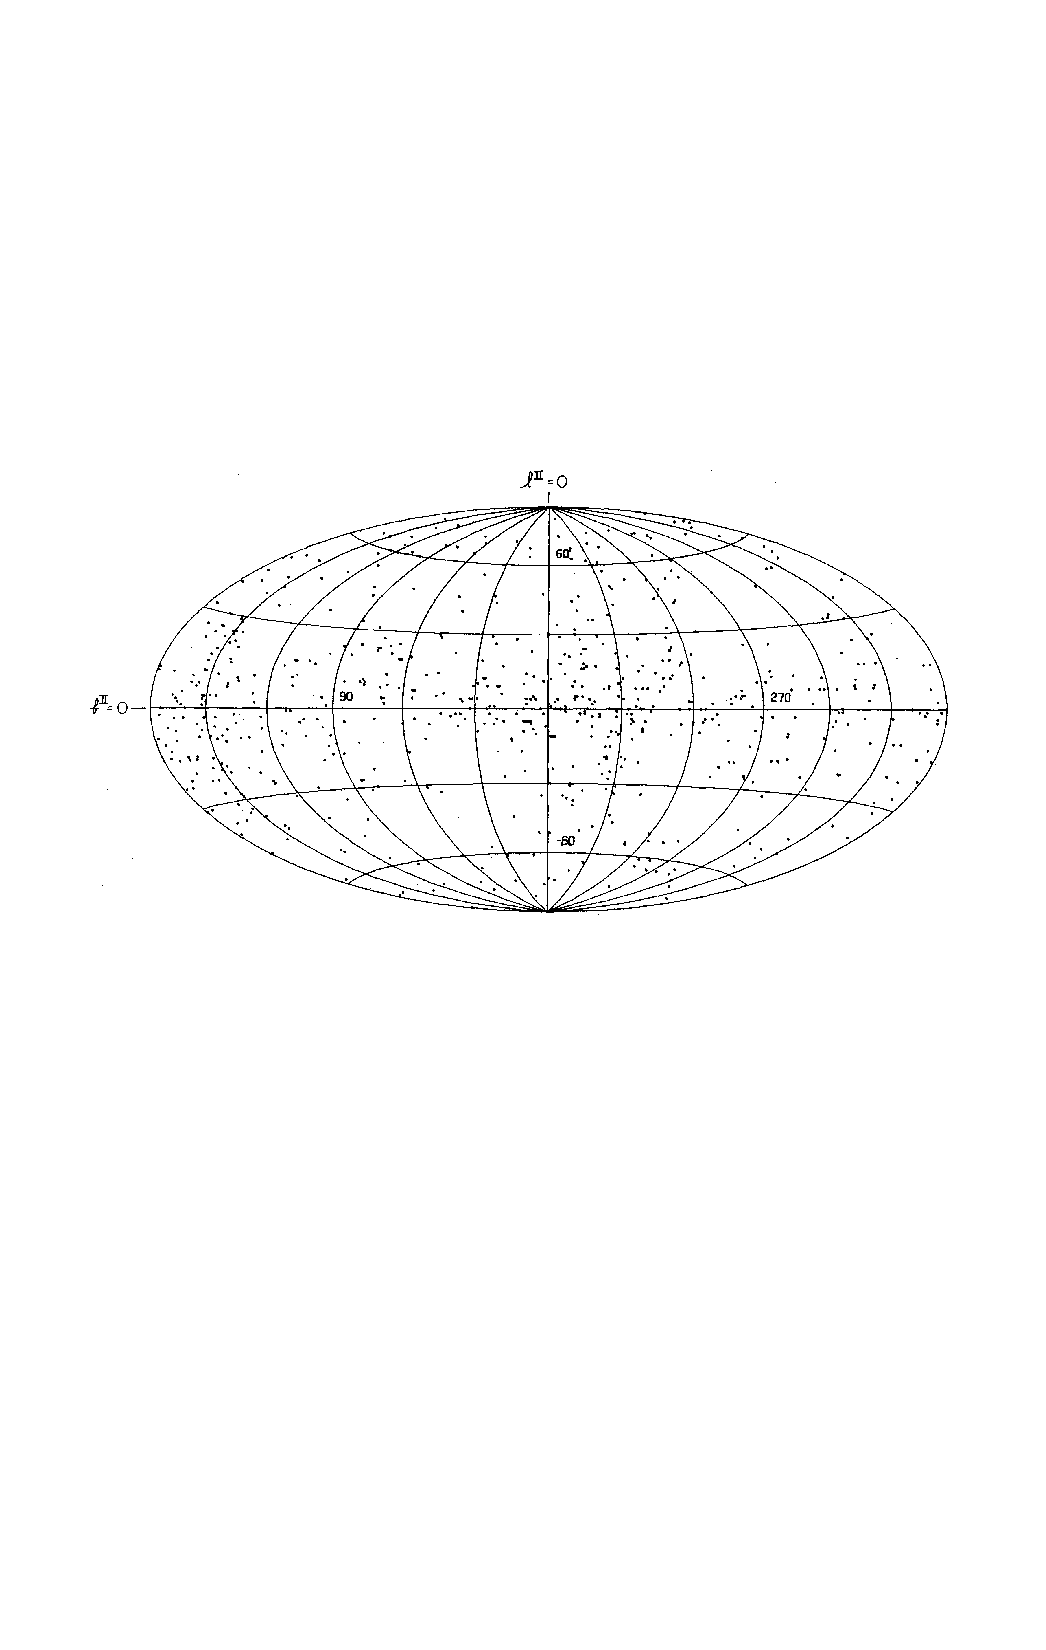
\includegraphics{chapters/introduction/figures/kraushaar_et_al_1972_skymap.pdf}
  \figlabel{oso3_skymap}
  \caption{The position of all 621 cosmic $\gamma$-rays
  detected by \ac{OSO-3}. This figure is from 
  \cite{kraushaar_1972_high-energy-cosmic}. }
\end{figure}



The major discovery by \ac{OSO-3} was confirmed by a balloon-based
$\gamma$-ray detector in 1970  \citep{kniffen_1970_study-gamma}.  In the
following year, the first $\gamma$-ray pulsar (the Crab) was detected
by another balloon-based detector \cite{browning_1971_detection-pulsed}.


% ``The field of gamma-ray astronomy took great leaps forward'' -- wikipedia

  % ``Additional gamma-ray experiments flew on the OGO, OSO, Vela, and Russian
  % Cosmos series of satellites. However, the first satellite designed as a
  % ``dedicated'' gamma-ray mission was the second Small Astronomy Satellite
  % (SAS-2) in 1972.`` - http://imagine.gsfc.nasa.gov/docs/science/know_l1/history_gamma.html

The next major advancement in $\gamma$-ray astronomy came 
\ac{SAS-2} and \cosb.

\Ac{SAS-2} was a dedicated $\gamma$-ray detector
launched by \ac{NASA} in November 15, 1972.  \ac{SAS-2} was
\cite{fichtel_1975_high-energy-gamma-ray} It improved upon \ac{OSO-3}
by incorporating a spark chamber and having an overall larger size.
The size of the active area of the detector was 640 $\cm^2$ and the
experiment had a much improved effective area of $\sim 115\unitspace cm^2$. The
spark chamber allowed for a separate measurement of the electron and
positron tracks, which allowed for improved directional reconstruction
of the incident $\gamma$-ray. \Ac{SAS-2} had a PSF $\sim5\degree$ at 30
\mev and $\sim1\degree$ at 1 \gev.

\Ac{SAS-2} collected data for over 6 months before a power supply
failure ended data collection. \Ac{SAS-2} Observed over 8,000
$\gamma$-ray photons covering $\sim55\%$ of
the sky including most of the Galactic plane.  
\Ac{SAS-2} discovered strong emission
along the Galactic plane and particularly towards the Galactic
cente. It also discovered
pulsations from the
Crab \citep{fichtel_1975_high-energy-gamma-ray} and Vela pulsar
\citep{thompson_1977_sas-2-high-energy}.  In addition, \ac{SAS-2}
discovered Geminga, the first $\gamma$-ray source with no compelling
multiwavelenth counterpart \citep{thompson_1977_final-sas-2}. Gemina
was eventually discovered to be a pulsar by \ac{EGRET}
\citep{bertsch_1992_pulsed-high-energy} and retroactively by \ac{SAS-2}
\citep{mattox_1992_observation-pulsed}.

% ``Cos-B was ESA's first satellite dedicated to a single experiment. Its
% scientific mission was to study in detail the sources of extra-terrestrial
% gamma radiation at energies above about 30 MeV. The originally foreseen
% duration of the mission was two years, but in fact Cos-B functioned
% successfully for 6 years and 8 months. During this time an extensive
% survey of the Galaxy was made in the energy range 50 MeV to 5 GeV.''
% -- http://sci.esa.int/science-e/www/area/index.cfm?fareaid=34

% ``Description Cos-B was the first ESA mission dedicated to the study of
% gamma-ray sources. Its results created a catalogue of these sources,
% known as the 2CG Catalogue, the first complete map of the gamma-ray
% emission from the disc of our Galaxy, the Milky Way, and the first
% detectable emission from an extra-galactic object 3C273.'' 
% -- http://www.esa.int/Our_Activities/Space_Science/Cos-B_factsheet

% cos b performance is described at:
%   http://www.rssd.esa.int/index.php?page=gr-tele&project=COSB

on August 9, 1975, \ac{ESA} launched \cosb, a $\gamma$-ray 
detector similar to \ac{SAS-2}. 
\cosb included a spark chamber but
improved upon the design of
\ac{SAS-2} by including a calorimeter below the spark chamber
which improved the energy resolution to $<100\%$ for energies $\sim
3\unitspace\gev$ \citep{bignami_1975_cos-b-experiment}.
\cosb has a comparable effective area to \ac{SAS-2}:
$\sim 50\unitspace\cm^2$ at $\sim400\unitspace\mev$
\citep{bignami_1975_cos-b-experiment}.  

\cosb operated successfully for over 6 years and produced the first
detailed catalog of the $\gamma$-ray sky.  In total, \cosb observed $\sim
80,000$ photons \cite{mayer-hasselwander_1982_large-scale-distribution}.
\Ac{2CG} detailed
the detection 25 $\gamma$-ray sources for $E>100\unitspace\mev$
\citep{swanenburg_1981_second-catalog}.  \figref{cos_b_skymap}
shows a map of these sources.  Of these sources, the vast majority
lay along the galactic plane and could not be positively identified
with sources observed at other wavelengths.  In addition, \cosb
observed the first ever extragalactic $\gamma$-ray source,
\citep[3C273,][]{swanenburg_1978_observation-high-energy}.

\begin{figure}[htb]
  \centering
  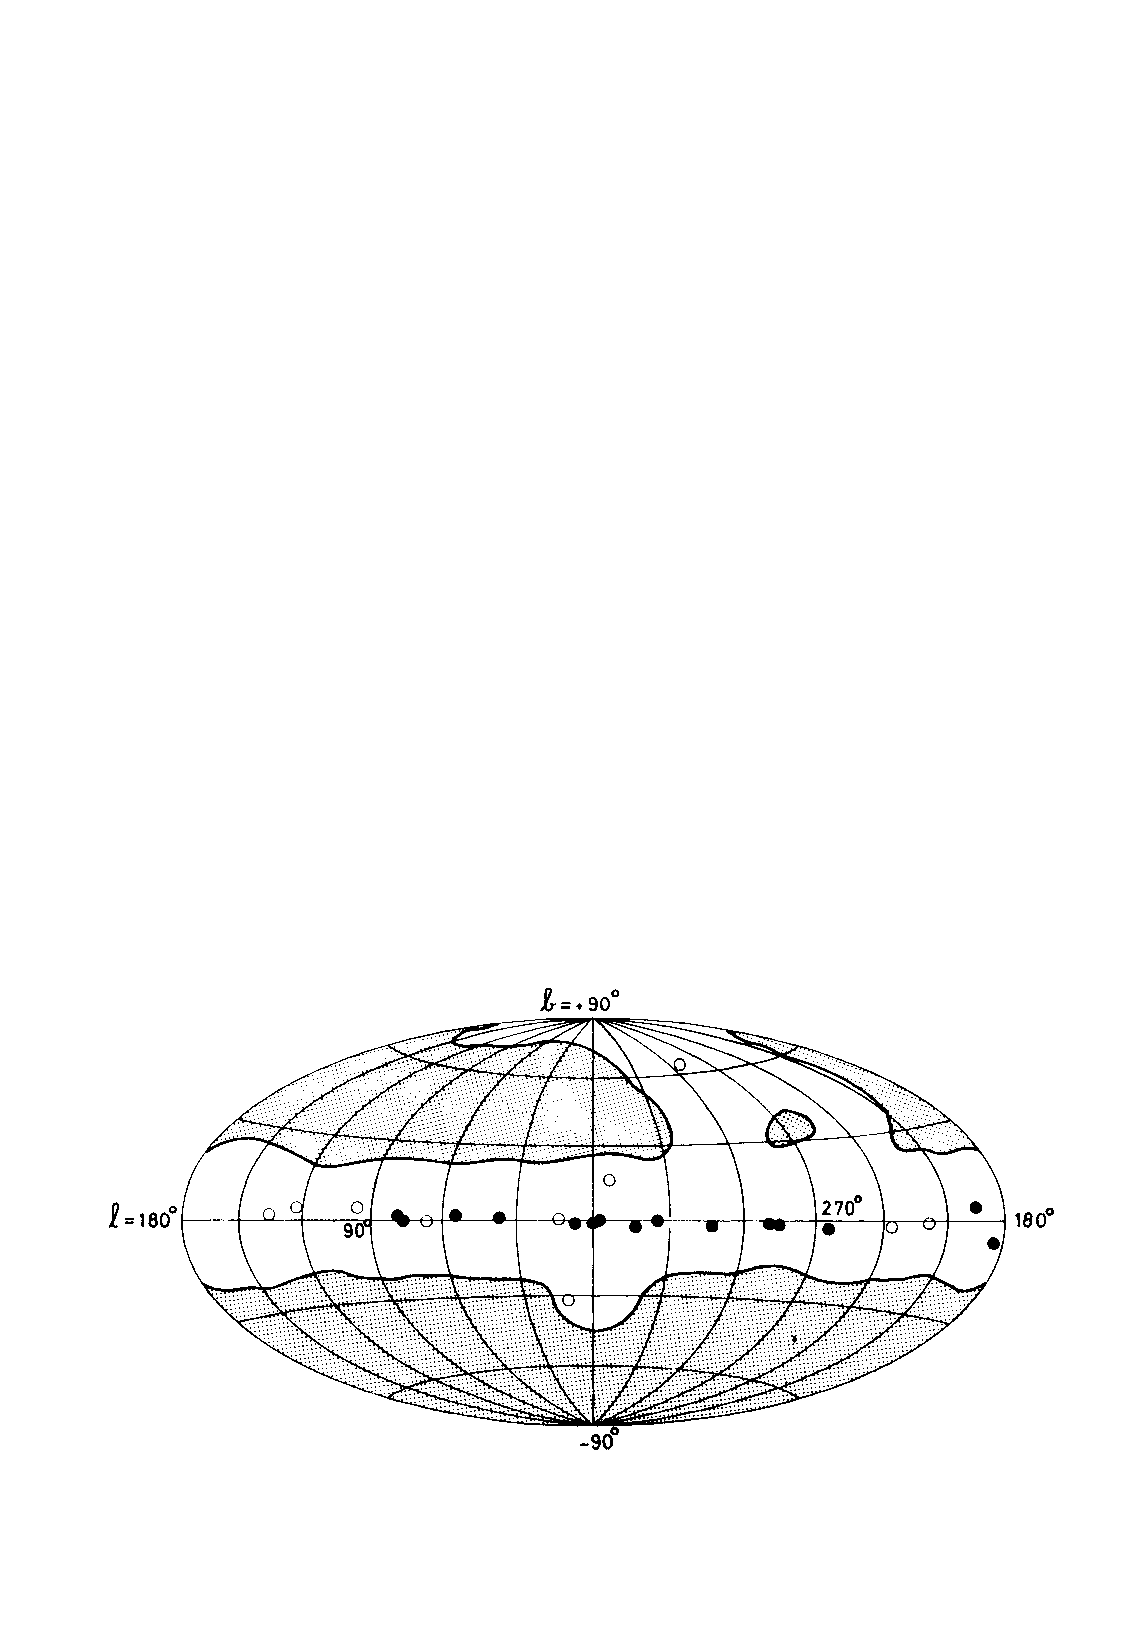
\includegraphics[width=\textwidth]{chapters/introduction/figures/cos_b_2nd_catalog.pdf}
  \figlabel{cos_b_skymap}
  \caption{
  A map of the sources observed by \cosb. The filled circles
  represent brighter sources. The unshaded region corresponds to
  the parts of the sky observed by \cosb.  This figure is from
  \cite{swanenburg_1981_second-catalog}.
  }
\end{figure}

% Good summary of EGRET Results:
%  http://arxiv.org/pdf/0811.0738.pdf

% EGRET: http://en.wikipedia.org/wiki/Energetic_Gamma_Ray_Experiment_Telescope
The next major $\gamma$-ray experiment was \ac{EGRET}.  It was
launched on board \ac{CGRO} in April , 1991.  \ac{CGRO}
was second of the Great Observatories satellites launched by
\acp{NASA}.  \ac{EGRET} had a design similar to \ac{SAS-2}, but had 
an expanded energy range, operating from
$20\unitspace\mev$ to $30\unitspace\gev$, an improved effective area
of $\sim1500\unitspace\cm^2$ from $\sim500\mev$ to $\sim1\unitspace\gev$, and an improved angular
resolution, decreasing to $\sim0.5\degree$ at its highest energies
\cite{thompson_1993a_calibration-energetic}.

At the time, \ac{CGRO} was the heaviest astrophysical experiment
launched into orbit, weighting $\sim17,000\unitspace\kg$. \ac{EGRET}
contributed $\sim6,000\unitspace\kg$ to the mass of \ac{CGRO}.

\ac{EGRET} vastly expanded the field of $\gamma$-ray astronomy.
\ac{EGRET} detected six pulsars \citep{nolan_1996a_egret-observations} and
also the Crab Nebula \cite{nolan_1993a_observations-pulsar}.  \ac{EGRET}
also detected the LMC, the first normal galaxy outside of our galaxy to
be detected at $\gamma$-rays \citep{sreekumar_1992a_observations-large}.
\ac{EGRET} also detected Centarus A, the first radio galaxy detected
at $\gamma$-rays \cite{sreekumar_1999a_emission-nearby}.  In total,
EGRET detected 271 $\gamma$-ray sources using 4 years.  The results were
presentted in \ac{3EG} \citep{hartman_1999a_third-egret}. This catalog
included 66 high confidence blazar identifications and 27 low-confidence
AGN identifications. \figref{third_egret_catalog_sources} plots
the position of the sources observed by \ac{EGRET}.

In total, \ac{EGRET} detected over 1,500,000 celestial gamma rays \cite{thompson_2008a_gamma-astrophysics:}.

\ac{EGRET} was designed with a 2 year mission lifetime, but operated for 9 years.
Over time, the performance of \ac{EGRET} degraded due to hardware failure
and due to having to replenish gas in the spark chamber \cite{esposito_1999a_in-flight-calibration}.


\todo[inline]{Get a picture of EGRET to include}

\begin{figure}[htb]
\centering
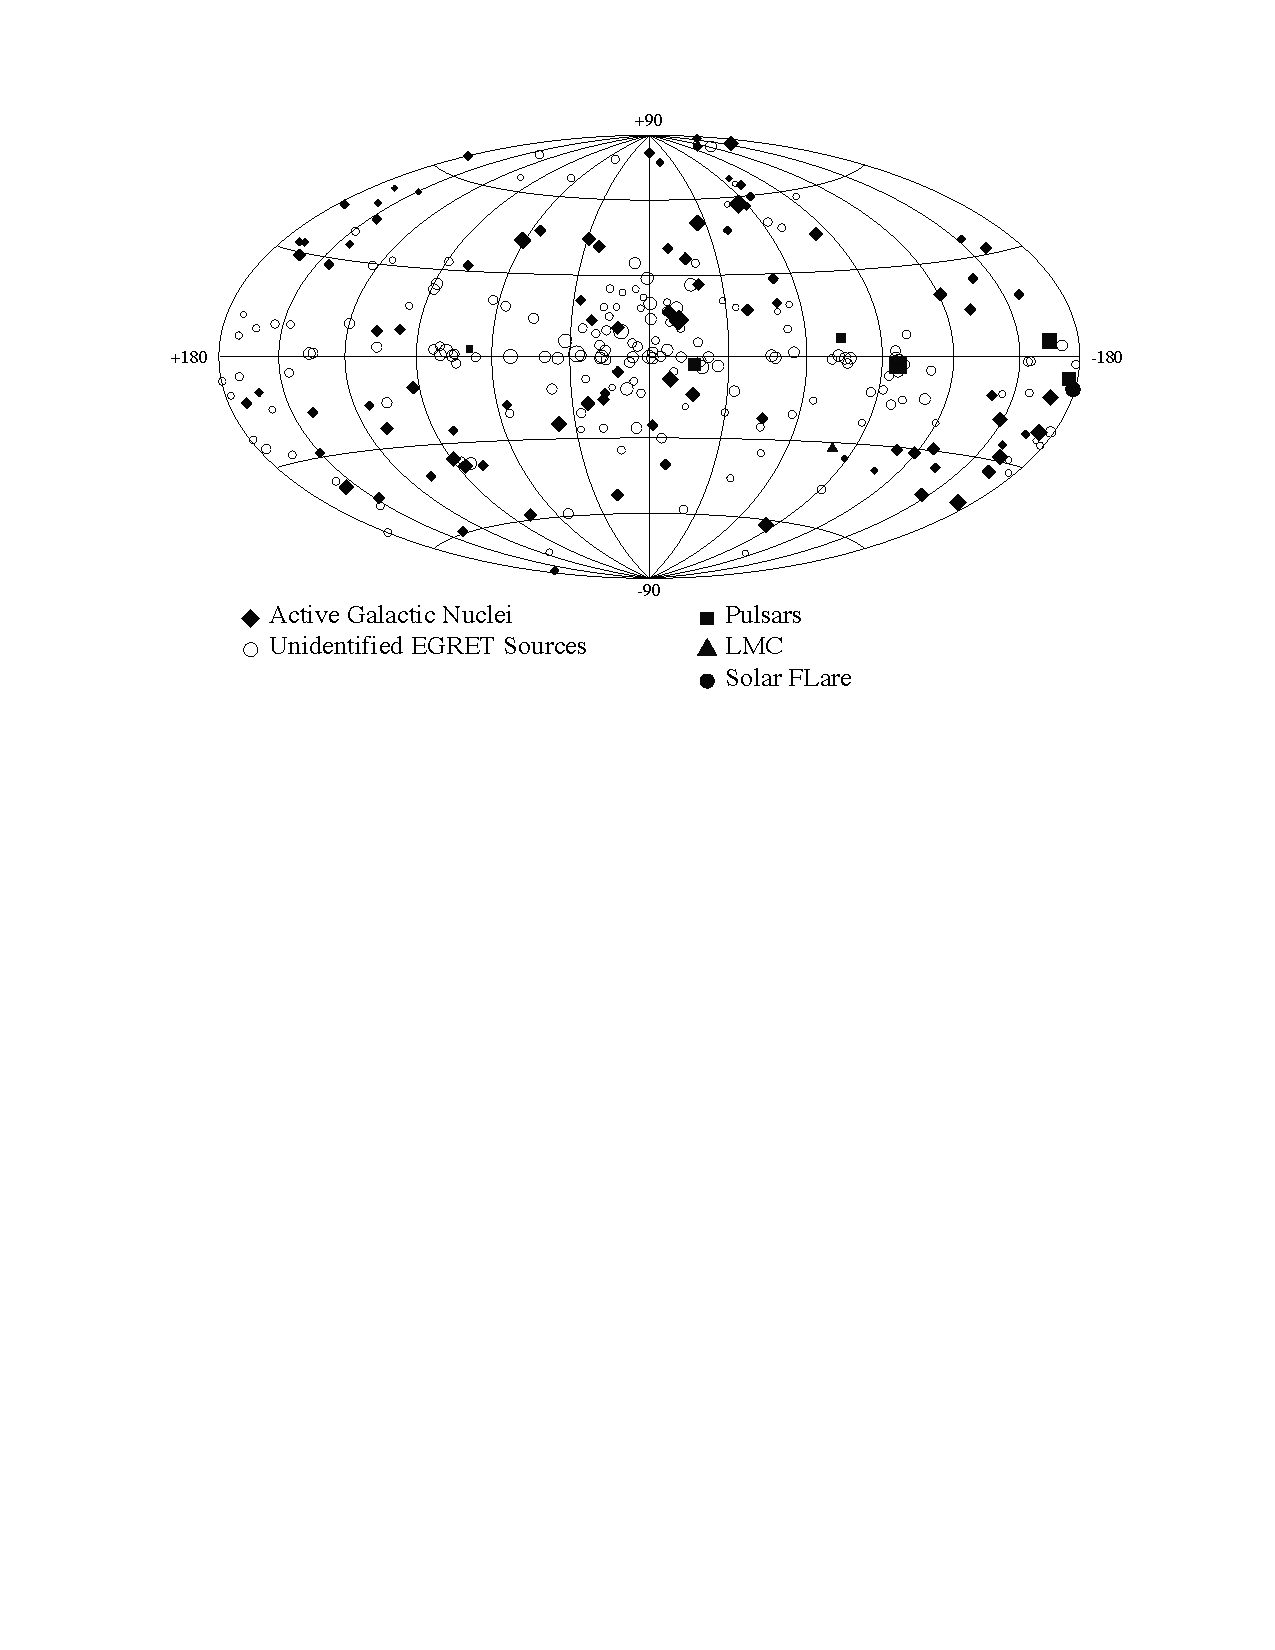
\includegraphics{chapters/introduction/figures/third_egret_catalog_sources.pdf}
\figlabel{third_egret_catalog_sources}
\caption{The position of \ac{EGRET} sources in the sky in galactic
coordinates.  The size of the source markers corresponds to the overall
source intensity.  This figure is from \citep{hartman_1999a_third-egret}.}
\end{figure}


\begin{itemize}
  \item AGILE
\item \fermi
  \item \todo[inline]{Short description of the history
    of TeV astronomy}

  \item A detailed description of \fermi detector will be presented in \secref{fermi_telescope}.
  \item The major source classes detected by \fermi will be presented in \secref{sources_detected_fermi} 


  The principles of the detector will be described in \secref{fermi_telescope}.
  \todo[inline]{What is the LAT effective area?}
\end{itemize}



